\documentclass{article}
\usepackage{listings}
\usepackage{graphicx}
\usepackage[slovene]{babel}
\usepackage{color}
\usepackage{amsmath}
\usepackage[usenames,dvipsnames]{xcolor}
\usepackage[hidelinks]{hyperref}
\usepackage{subcaption}
\usepackage{float}
\usepackage{rotating} 
\usepackage{hyperref}
\usepackage{caption}
\graphicspath{{./images/}}

\newcommand{\Ai}{\mathrm{Ai}}
\newcommand{\Bi}{\mathrm{Bi}}
\newcommand{\dd}{\,\mathrm{d}}


\begin{document}

\title{Matematično-fizikalni praktikum \\[3mm] \large Naloga 1}
\author{Luka Papež}
\date{10.\ oktober 2024}

\begin{center}
    
\includegraphics[width=8cm]{logo-fmf.png}
\end{center}

{
    \let\newpage\relax
    \maketitle
}

\maketitle
\newpage
\section{Naloga}
{\sl Naloga:} Z uporabo kombinacije Maclaurinove vrste in asimptotskega
razvoja poišči čim učinkovitejši postopek za izračun
vrednosti Airyjevih funkcij $\Ai$ in $\Bi$ na vsej real\-ni osi
z {\bf absolutno} napako, manjšo od $10^{-10}$. Enako naredi tudi z {\bf relativno} napako in ugotovi,
ali je tudi pri le-tej dosegljiva natančnost, manjša od $10^{-10}$.
Pri oceni napak si po\-ma\-gaj s programi, ki znajo računati s poljubno
natančnostjo, na primer z {\sc Mathematico} in/ali paketi {\sc mpmath} in {\sc decimal} v programskem
jeziku {\sc Python}. \\ 

\noindent {\sl Dodatna naloga:} Ničle funkcije $\Ai$ pogosto srečamo v matematični
analizi pri določitvi intervalov ničel specialnih funkcij
in ortogonalnih polinomov \cite{1_szego} ter v fiziki pri računu
energijskih spektrov kvantnomehanskih sistemov \cite{1_landauQM}.
Poišči prvih sto ničel $\{a_s\}_{s=1}^{100}$ Airyjeve
funkcije $\Ai$ in prvih sto ničel $\{b_s\}_{s=1}^{100}$
funkcije $\Bi$ pri $x<0$ ter dobljene vrednosti primerjaj s podanima formulama.

\section{Uvod}
Airyjevi funkciji $\Ai$ in $\Bi$ (slika~\ref{sl:airy})
se v fiziki pojavljata predvsem v optiki in kvantni mehaniki
\cite{1_vallee}.  Definirani sta kot neodvisni rešitvi enačbe
%
\begin{equation*}
  y''(x) -xy(x) = 0
\end{equation*}
%
in sta predstavljivi v integralski obliki
%
\begin{equation*}
  \Ai(x) = \frac{1}{\pi} \int_0^\infty \cos (t^3/3 + x t) \dd t \>,\quad
  \Bi(x) = \frac{1}{\pi} \int_0^\infty \left[ \mathrm{e}^{-t^3/3 + x t}
  + \sin (t^3/3 + x t) \right] \dd t \>.
\end{equation*}
%

\begin{figure}[hbtp]
\begin{center}
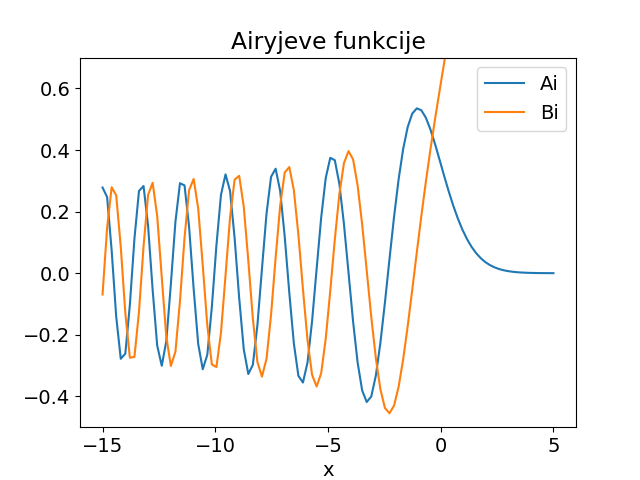
\includegraphics[width=11cm]{both_funcs.png}
\end{center}
\vspace*{-7mm}
\caption{Graf Airyevih funkcij $\Ai$ in $\Bi$ za realne
argumente.  Funkcija $\Ai$ je povsod omejena,
medtem ko $\Bi$ divergira na pozitivni polosi.
Ni"cle imata le na negativni polosi.}
\label{sl:airy}
\end{figure}

Za majhne $x$ lahko funkciji $\Ai$ in $\Bi$ izrazimo
z Maclaurinovima vrstama
%
\begin{equation*}
  \Ai(x) = \alpha f(x) - \beta g(x)\>,\qquad
  \Bi(x) = \sqrt{3}\, \Bigl[\alpha f (x) + \beta g(x) \Bigr]\>,
\end{equation*}
kjer v $x=0$ veljata zvezi
%
$\alpha = \Ai(0) = \Bi(0)/\sqrt{3}\approx 0.355028053887817239$ in
$\beta = -\Ai'(0) = \Bi'(0)/\sqrt{3}\approx 0.258819403792806798$.
Vrsti za $f$ in $g$ sta
\begin{equation*}
  f(x) = \sum_{k=0}^\infty
  \left(\frac{1}{3}\right)_k \frac{3^k x^{3k}}{(3k)!} \>, \qquad
  g(x) = \sum_{k=0}^\infty
  \left(\frac{2}{3}\right)_k \frac{3^k x^{3k+1}}{(3k+1)!} \>,
\end{equation*}
kjer je
\begin{equation*}
  (z)_n = \Gamma(z+n)/\Gamma(z) \>, \qquad (z)_0 = 1 \>.
\end{equation*}

Za velike vrednosti $|x|$ Airyjevi funkciji aproksimiramo
z njunima asimp\-tot\-ski\-ma razvojema.  Z novo spremenljivko
$\xi=\frac{2}{3} |x|^{3/2}$ in asimptotskimi vrstami
%
\begin{equation*}
  L(z) \sim \sum_{s=0}^\infty \frac{u_s}{z^s}\>,\qquad
  P(z) \sim \sum_{s=0}^\infty (-1)^s \frac{u_{2s}}{z^{2 s}}\>,\qquad
  Q(z) \sim \sum_{s=0}^\infty (-1)^s \frac{u_{2s+1}}{z^{2 s+1}}\>,
\end{equation*}
s koeficienti
\begin{equation*}
u_s = \frac{ \Gamma(3s + \frac{1}{2})}
        {54^s s!\, \Gamma(s + \frac{1}{2}) }
\end{equation*}
za velike pozitivne $x$ izrazimo
%
\begin{equation*}
\Ai(x)\sim  \frac{\mathrm{e}^{-\xi}}{2\sqrt{\pi} x^{1/4}} \, L(-\xi) \>, \qquad
\Bi(x)\sim  \frac{\mathrm{e}^{\xi}} { \sqrt{\pi} x^{1/4}} \, L(\xi)\>,
\end{equation*}
%
za po absolutni vrednosti velike negativne $x$ pa
%
%
\begin{align*}
    \Ai(x)&\sim  \frac{1}{\sqrt{\pi} (-x)^{1/4}}
    \Bigl[ \phantom{-}\sin(\xi-\pi/4) \, Q(\xi)
                    + \cos(\xi-\pi/4) \, P(\xi)\Bigr] \>, \\
    \Bi(x)&\sim  \frac{1}{\sqrt{\pi} (-x)^{1/4}}
    \Bigl[ - \sin(\xi-\pi/4) \, P(\xi)
      + \cos(\xi-\pi/4) \, Q(\xi)\Bigr]\>.
\end{align*}
\newpage
\section{Rešitev}

\subsection{Taylorjeva vrsta}
Za pristop k nalogi bomo najprej implementirali Taylorjevo vrsto, saj je ta precej enostavnejša kot asimptotska vrsta. Vrsta podana v uvodu je precej računsko intenzivna zato jo poskusimo najprej poenostaviti. Pogledamo funkciji $f$ in $g$ iz katerih sta sestavljeni funkciji $\Ai$ in $\Bi$.
\begin{equation*}
  f(x) = \sum_{k=0}^\infty
  \left(\frac{\Gamma(k + 1/3)}{\Gamma(1/3)}\right) \frac{3^k x^{3k}}{(3k)!} \>, \qquad
  g(x) = \sum_{k=0}^\infty
  \left(\frac{\Gamma(k + 2/3)}{\Gamma(2/3)}\right) \frac{3^k x^{3k+1}}{(3k+1)!} \>,
\end{equation*}
Spomnimo se relacije $\Gamma(n+1)=n\Gamma(n)$. Iz tega lahko opazimo, da lahko člene $f$ in $g$ zapišemo v rekurzivni obliki. Označimo člene vrste $f$ z $a_k$ in člene vrste $g$ z $b_k$. Potem velja:
\begin{equation*}
    a_{k+1} = \frac{x^3}{(3k + 3)(3k + 2)} a_k \>, \qquad
    b_{k+1} = \frac{x^3}{(3k + 4)(3k + 3)} b_k \>,
\end{equation*}
Za izračun vrste pa potrebujemo še prva elementa funkcij $a_0=1$ in $b_0=x$. \\
Najprej preverimo, če se naša vrsta vizualno ujema z vrednostmi funkcij $\Ai$ in $\Bi$.
\begin{figure}[H]
    \centering
    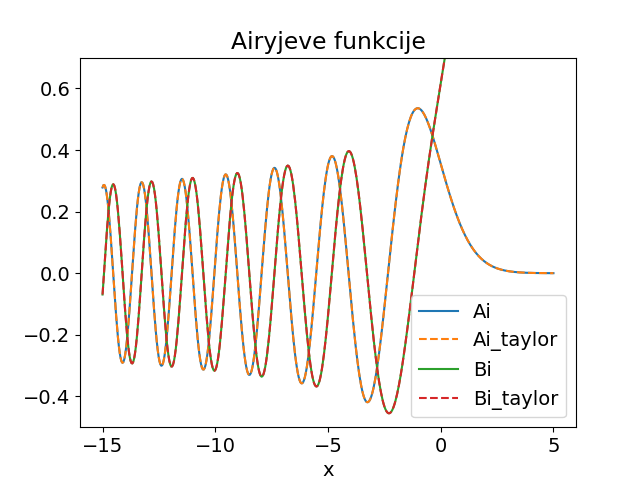
\includegraphics[width=0.8\textwidth]{taylor_comparison.png}
    \caption{Primerjava Taylorjeve vrste in dejanskih vrednosti funkcij $\Ai$ in $\Bi$}
\end{figure}
Naše vrste se dobro ujemajo z vrednostmi funkcij $\Ai$ in $\Bi$ za majhne vrednosti $x$. Zdaj narišemo grafa z relativno in absolutno napako s 300 členi taylorjeve vrste.
\begin{figure}[H]
    \centering
    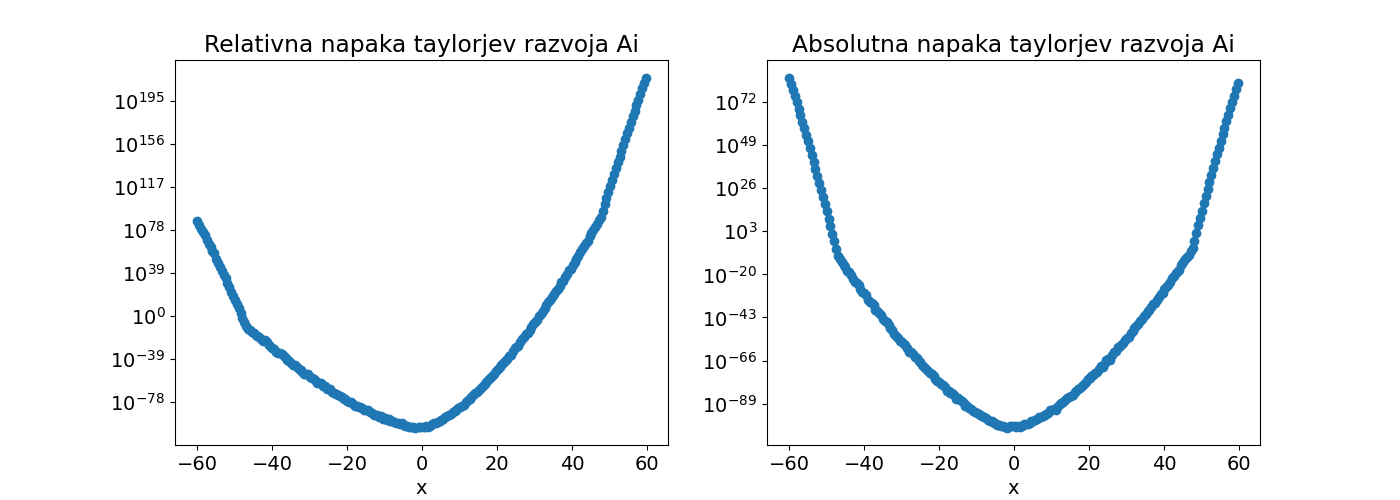
\includegraphics[width=1.1\textwidth]{Ai_taylorjev_razvoj.png}
    \caption{Napake Taylorjeve vrste pri izračunu funkcije $\Ai$}
\end{figure}
\begin{figure}[H]
    \centering
    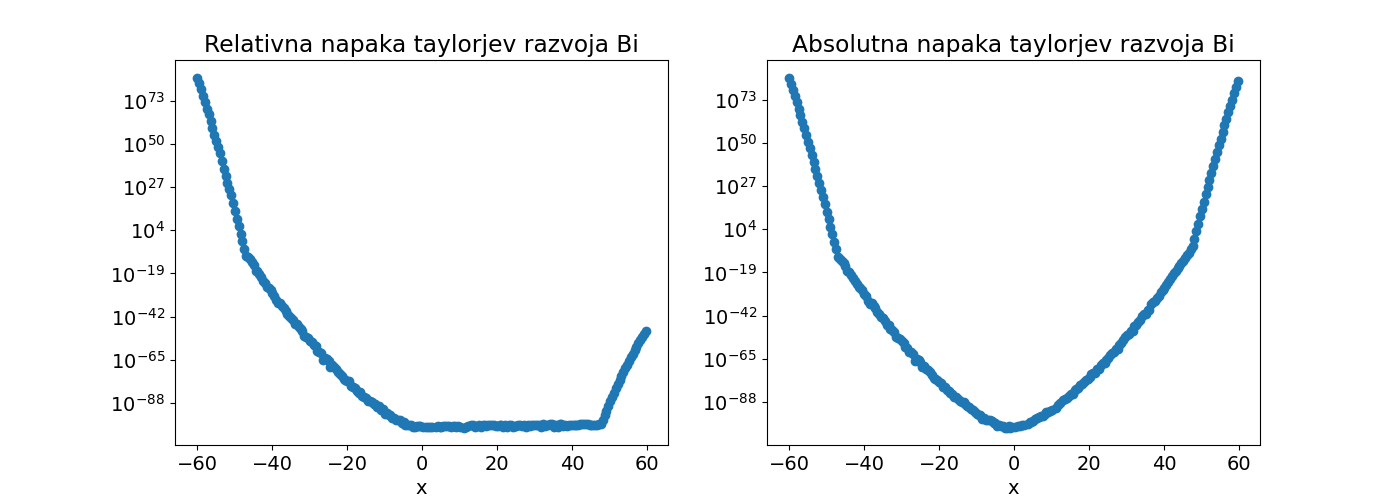
\includegraphics[width=1.1\textwidth]{Bi_taylorjev_razvoj.png}
    \caption{Napake Taylorjeve vrste pri izračunu funkcije $\Bi$}
\end{figure}
Absolutne napake so simetrične okoli ničle. Kar pa ne velja pri relativni napaki funkcije predvsem pri $\Bi$. To odstopanje lahko pojasnimo z zelo hitro divergenco funkcije $\Bi$ na pozitivni polosi. Za zaključek o Taylorjevi vrsti si poglejmo še kako se spreminja vsota napake na območjo $-20$ do $20$ s številom členov.
\begin{figure}[H]
    \centering
    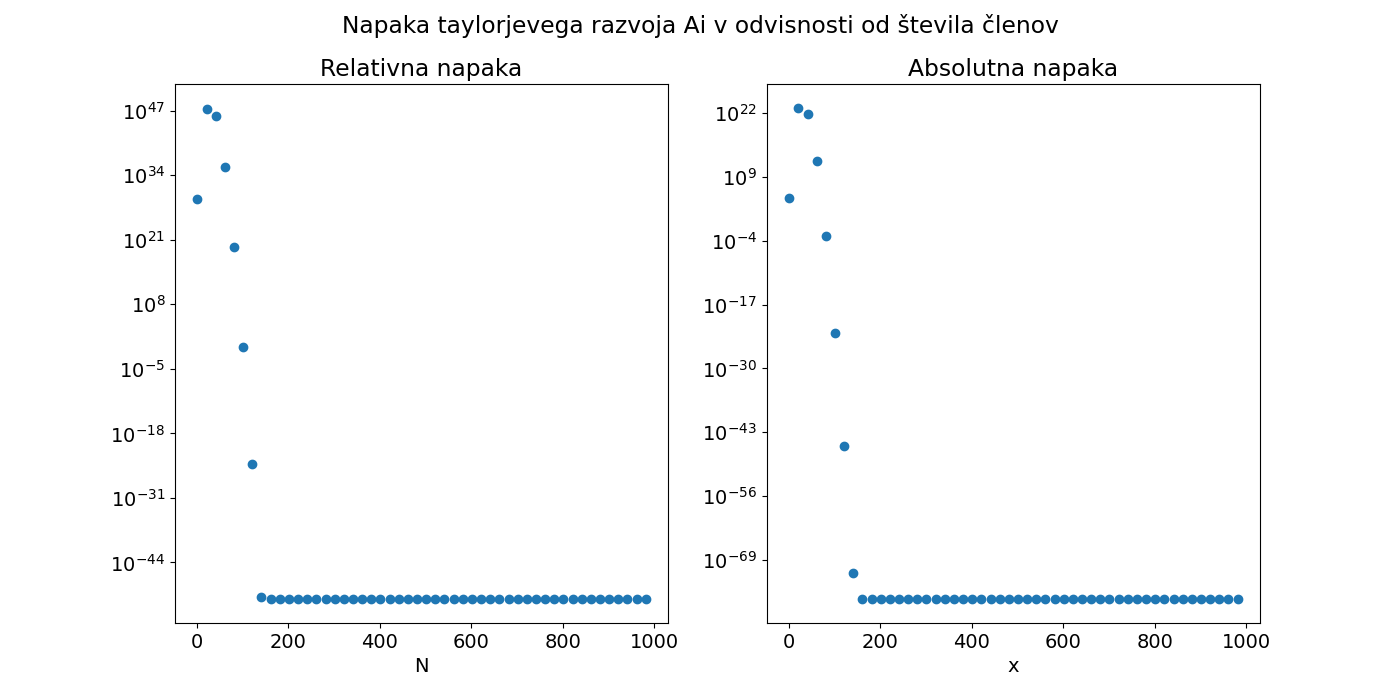
\includegraphics[width=1.1\textwidth]{taylor_cleni_Ai.png}
    \caption{Napake Taylorjeve vrste pri N členih}
\end{figure}
Odvisnost napake od števila členov je lepo razvidna. Graf pa je praktično enak za obe funkciji zato je tukaj prikazan le za funkcijo $\Ai$. Napaka pada do približno $N=200$ potem pa se ustali zato bomo v nadaljevanju uporabljali 300 členov.
\subsection{Asimptotska vrsta}
Asimptotska vrste je sestavljena iz treh vrst $L$, $P$ in $Q$. Za izračun teh vrst potrebujemo koeficiente $u_s$. Poenostavimo koeficient $u_s$ po postopku, ki smo ga že uporabili pri Taylorjevi vrsti.
\begin{equation*}
    u_{s+1} = \frac{(6s + 5)(6s + 1)}{72} u_s
\end{equation*}
Pomembna opazka pa je tudi, da je koeficient $u_s$ odvisen le od $s$. Zato lahko vse koeficiente izračunamo le enkrat in jih nato uporabljamo za izračun vseh treh vrst. Še eno pomembno dejstvo o asimptotskih vrstah pa je, da te divergirajo. Zato namesto vsot s fiksnim številom členov, v tem delu prištevamo člene dokler ti ne začnejo naraščati. \\

Zdaj bomo preskočili vizualno primerjavo in si le ogledali kako se obnašajo napake pri asimptotski vrsti.
\begin{figure}[H]
    \centering
    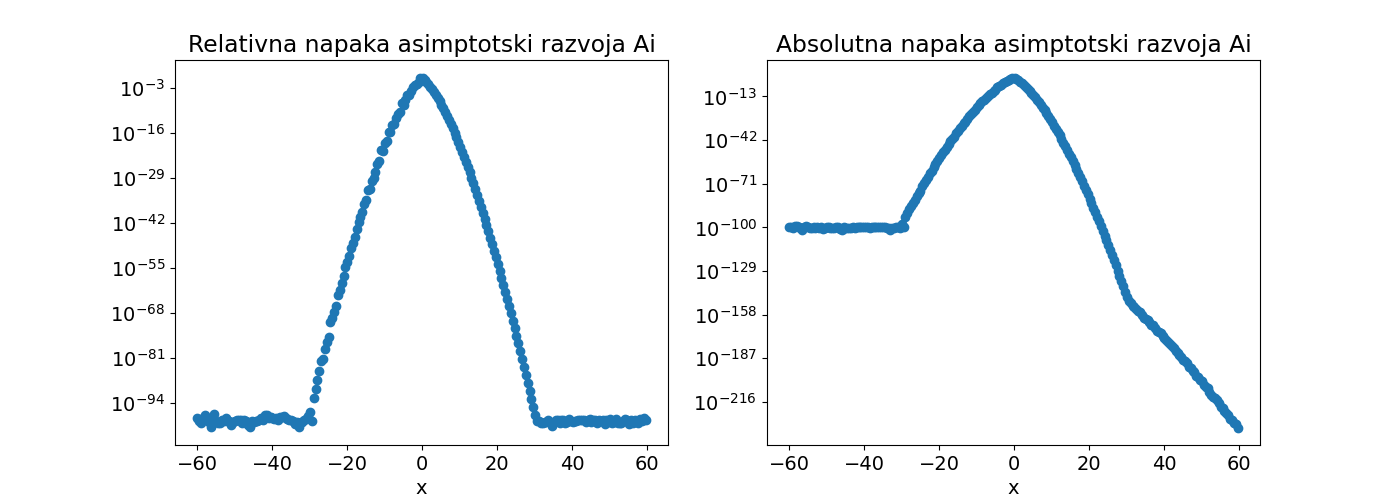
\includegraphics[width=1.1\textwidth]{Ai_asimptotski_razvoj.png}
    \caption{Napake asimptotske vrste funkcije $\Ai$}
\end{figure}
\begin{figure}[H]
    \centering
    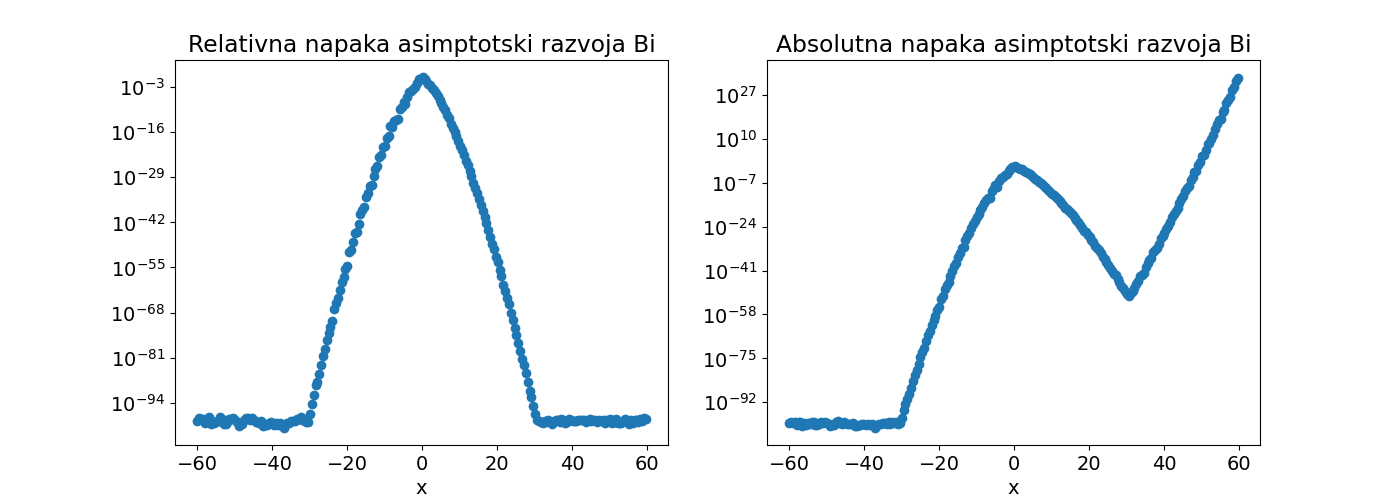
\includegraphics[width=1.1\textwidth]{Bi_asimptotski_razvoj.png}
    \caption{Napake asimptotske vrste funkcije $\Bi$}
\end{figure}
V tem primeru je relativna napaka precej ne zanimiva in po pričakovanjih narašča, ko preidemo v področje manjših števil. Pri absolutni napaki pa opazimo nenadne prelome na pozitivni polosi. To je posledica nastavljene velikosti števil v spominu. Saj se funkciji $\Bi$ zelo hitro začnejo povečevati števila in zato nima dovolj spomina, da bi se ohranila vse števke. Funkcija $\Ai$ pa konvergira k ničli in za razliko od $\Bi$ se števila in hkrati absolutna napaka zmanjšujejo.
\subsection{Združitev obeh vrst}
Zdaj ko imamo implementirani obe vrsti lahko njuni lastnosti uporabimo za natančnejši izračun vrednosti funkcij $\Ai$ in $\Bi$. Za majhne vrednosti uporabimo Taylorjevo vrsto, za velike pa asimptotsko. Preostane nam le še določitev meje za prehod. Združimo grafa napak obeh vrst.
\begin{figure}[H]
    \centering
    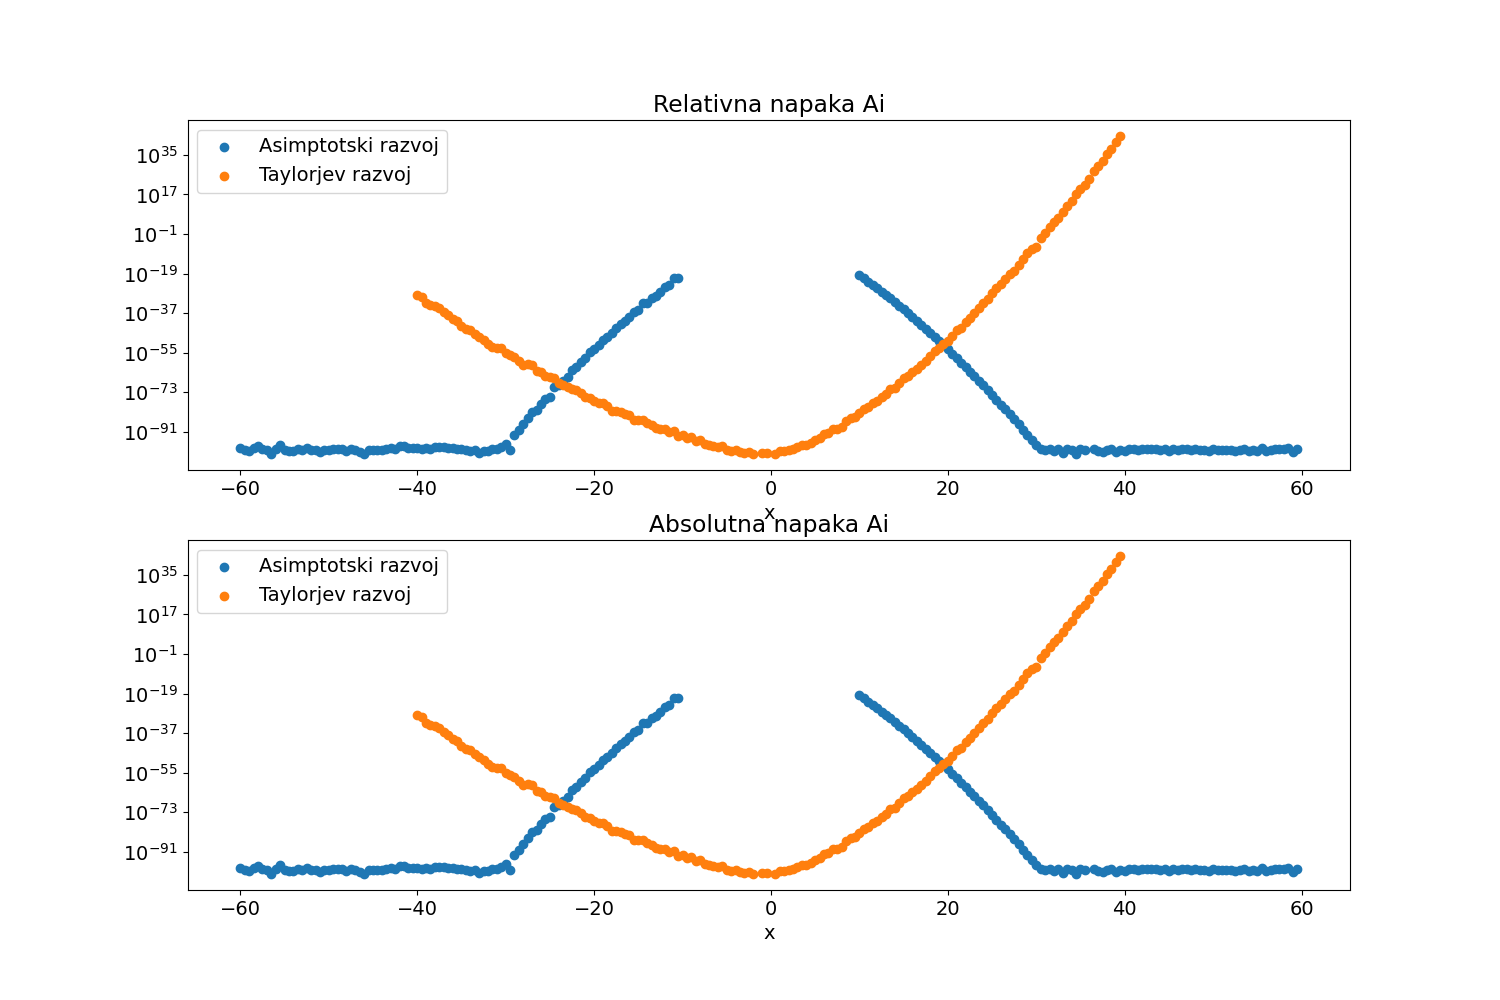
\includegraphics[width=1\textwidth]{primerjava_razvojev_Ai.png}
    \caption{Napake pri izračunu funkcije $\Ai$}
\end{figure}
\begin{figure}[H]
    \centering
    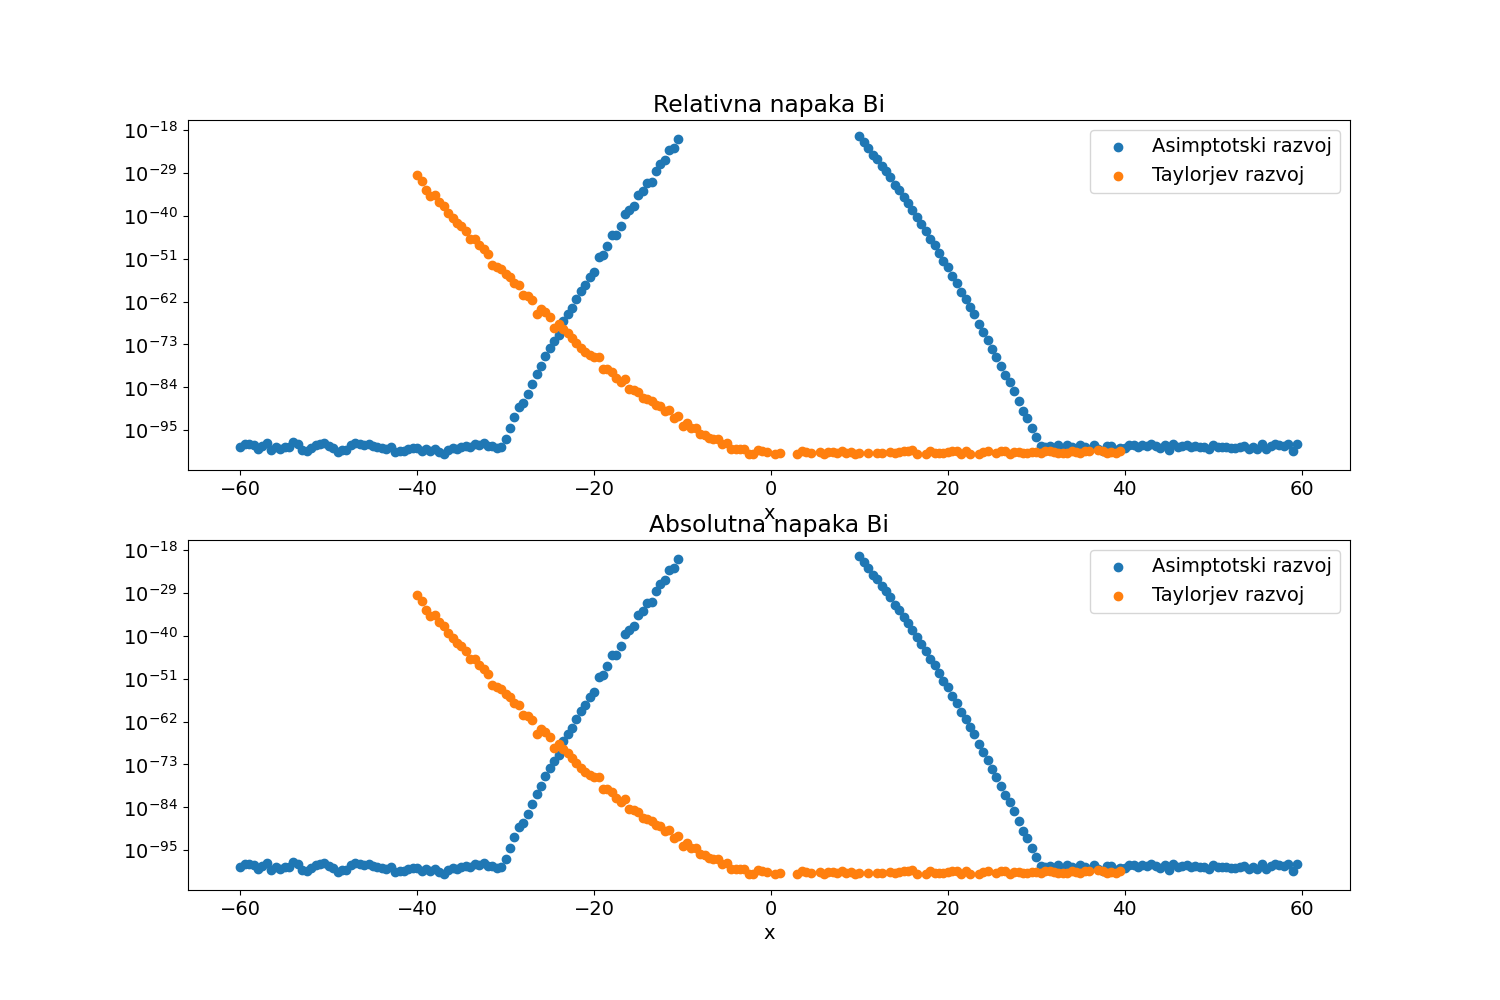
\includegraphics[width=1\textwidth]{primerjava_razvojev_Bi.png}
    \caption{Napake pri izračunu funkcije $\Bi$}
\end{figure}
\newpage
Iz zgornjih grafov je razvidno, da je najbolj primerna skupna meja za prehod $x=30$. Iz vrednosti napak pa lahko tudi sklepamo, da smo dosegli zahtevano natančnost $10^{-10}$. K temu zaključku spada še komentar, da jo lahko dosežemo le, če izberemo primerno natančnost števil glede na velikost števil s katerimi računamo($dps$ nastavitev v knjižnici $mpmath$).
\section{Dodatna naloga}
V dodatni nalogi najprej uporabimo \emph{in-built} funkcije za izračun ničel funkcij $\Ai$ in $\Bi$. Nato pa uporabimo še podani formuli s pomočjo prvih petih členov asimptotske vrste funkcije $f$ \cite{1_abram}. 
%
\begin{equation*}
    a_s = - f \left( \frac{3\pi(4s-1)}{8} \right) \>, \qquad
    b_s = - f \left( \frac{3\pi(4s-3)}{8} \right) \>, \qquad s = 1,2,\ldots \>,
\end{equation*}
%
\begin{equation*}
f(z) \sim z^{2/3} \left(
1 + \frac{5}{48} \, z^{-2}
-\frac{5}{36} \, z^{-4}
+\frac{77125}{82944} \, z^{-6}
-\frac{108056875}{6967296} \, z^{-8} + \ldots\right) \>.
\end{equation*}
Za primerjavo formule in dejanskih vrednosti si oglejmo graf napak. 
\begin{figure}[H]
    \centering
    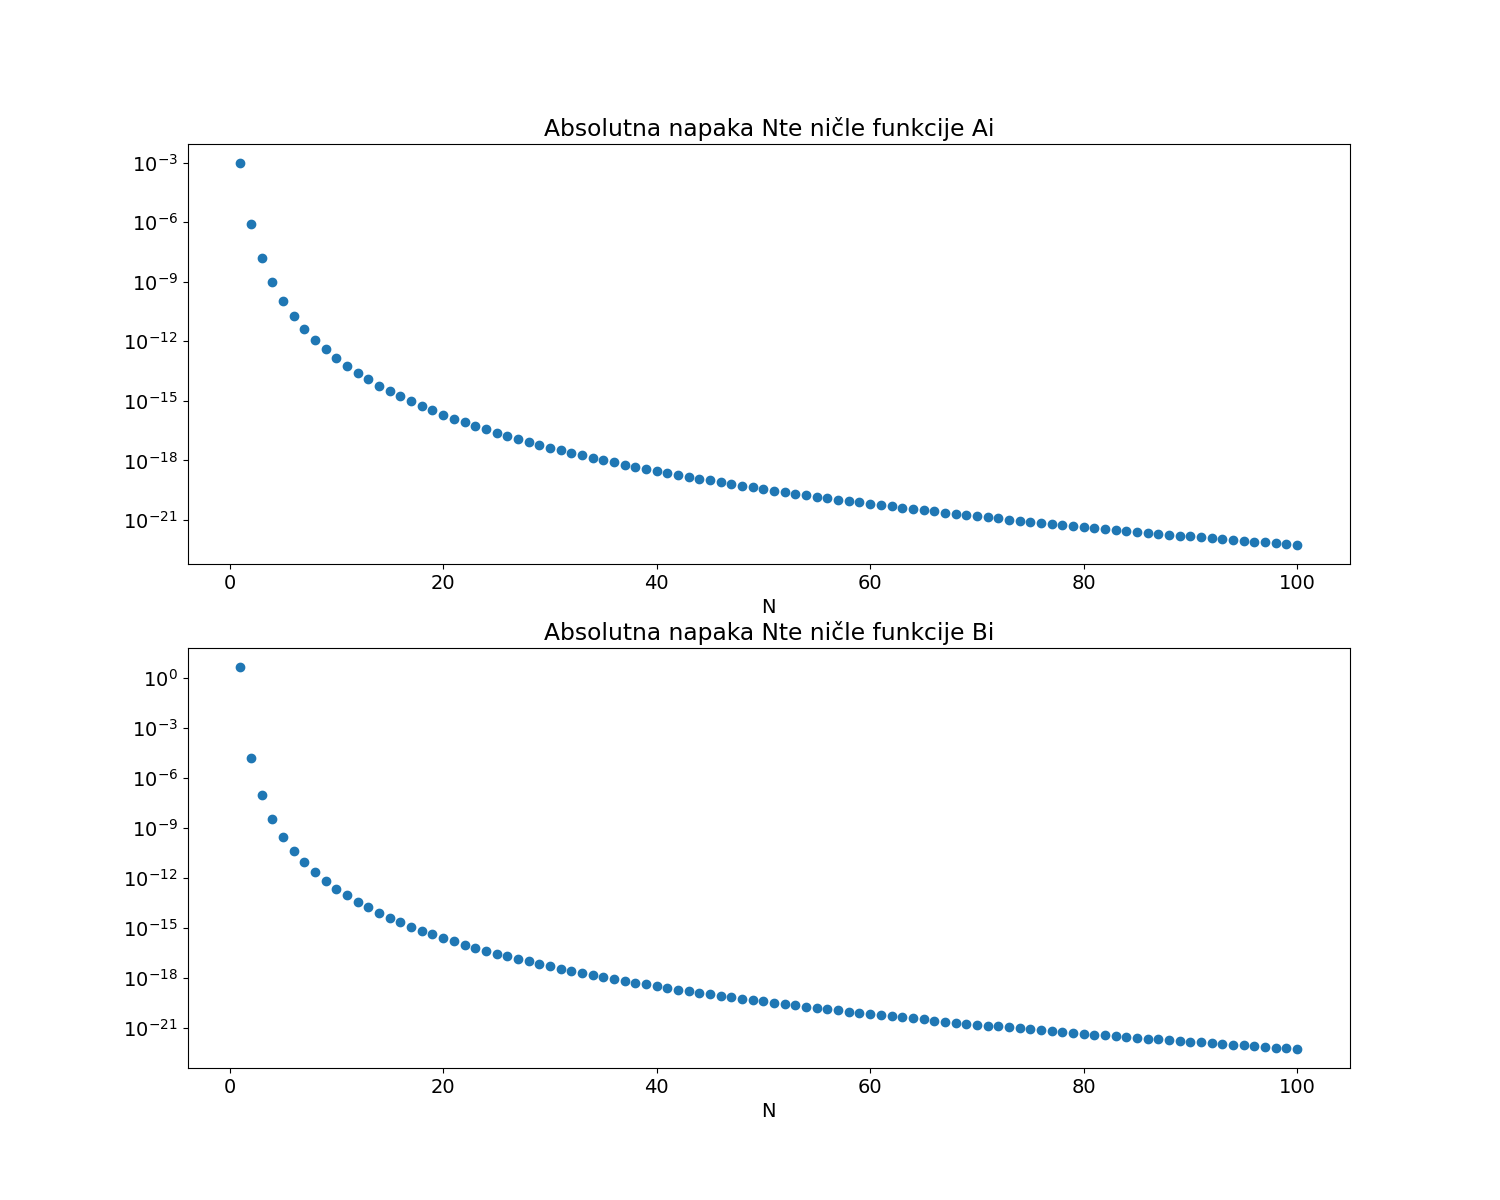
\includegraphics[width=1.1\textwidth]{zeros.png}
    \caption{Napake pri izračunu ničel funkcije $\Ai$ s pomočjo vrste funkcije f}
\end{figure}
Absolutne napake padajo s številom ničle. To dejstvo lahko pričakujemo iz izgleda funkcij in dejstva, da smo uporabili asimptotsko vrsto. Saj imata Airyjevi funkciji ničle le na negativni polosi in napaka asimptotske vrste pada z naraščanjem števil.
\section{Zaključek}
Dosegli smo cilj naloge, ki je bil implementacija numeričnega računanja Airjevih funkcij z absolutnimi in relativnimi napakami manjšimi od $10^{-10}$. Za doseg tega cilja smo uporabili kombinacijo Taylorjeve in asimptotske vrste. Ideja naloge mi je bila zanimiva, saj nisem imel prejšnjih izkušenj z zelo natančnim računanjem. Sem pa imel kar precej težav z implementacijo asimptotske vrste zaradi površnosti pri prepisovanju formul. 
\begin{thebibliography}{99}
    \setlength{\itemsep}{.2\itemsep}\setlength{\parsep}{.5\parsep}
    \bibitem{1_vallee} O.~Vall\'ee, M. Soares,
      {\sl Airy functions and applications to physics},
      Imperial College Press, London 2004.
    \bibitem{1_szego} G.~Szeg\"o, {\sl Orthogonal polynomials},
      AMS, Providence 1939.
    \bibitem{1_landauQM} L.~D.~Landau, E.~M.~Lifshitz, {\sl Course in
      theoretical physics, Vol.~3: Quantum mechanics},
      $3^\mathrm{rd}$ edition, Pergamon Press, Oxford 1991.
    \bibitem{1_abram} M.~Abramowitz, I.~A.~Stegun, {\sl Handbook of mathematical
      functions}, $10^\mathrm{th}$ edition, Dover Publications, Mineola 1972.
    \bibitem{wikipedia} Procyon117, Schneelocke, {\sl Airy function}, Wikipedia, 2024.
    \bibitem{1_manton} N.~S.~Manton, {\sl Asymptotic methods}, 
    Mathematical Tripos Part II, 2012
\end{thebibliography}

\end{document}
